
\documentclass{ecai}
\usepackage{graphicx}
\usepackage{latexsym}
\usepackage{booktabs}
\usepackage{caption}
\usepackage{subcaption}

\title{Cross-Lingual Intent Classification using BERT: A Multilingual Approach}

\author{
Abhishek Gupta \and
Bharat Karthi R K \and
Gayathri Ramasubramaniyam \and
Harikrishnan C \and
Indrerjit Singh Chahuan \and
Monika Tyagi
\institute{Team from DA 225o Deep Learning (Summer 2025), Indian Institute of Science}
}

\begin{document}
\maketitle

\begin{abstract}
With conversational AI taking center stage in the world, systems such as chatbots, conversation commerce, virtual assistants, and customer support are required to function across multiple languages. This makes multilingual intent classification a critical task. This project explores the use of the transformer model BERT for intent classification across various languages. The project aims to classify user intents using pre-trained multilingual BERT (mBERT) in a multi-language dataset including English, Spanish, French, and Hindi. The model's performance is evaluated using accuracy, precision, recall, and F1-score. The result is a robust classifier capable of improving accessibility and accuracy in multilingual AI applications.
\end{abstract}

\section{Introduction}
Multilingual intent classification is crucial for natural language understanding in applications like customer support, voice assistants, and conversational AI. Language diversity and data sparsity pose major challenges for scalable NLP models. We propose a multilingual BERT-based solution trained and evaluated on a rich multilingual dataset.

\section{System Architecture}
The system uses mBERT with a fine-tuned classification head. Inputs are tokenized to 128-token sequences and passed through mBERT, followed by a softmax classifier over intent labels.

\begin{figure}[h]
\centering
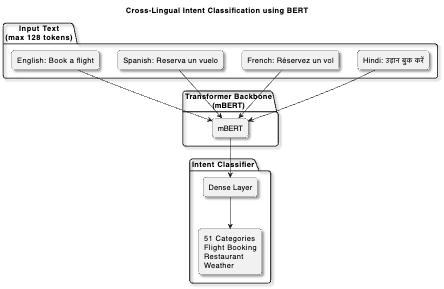
\includegraphics[width=0.8\linewidth]{architecture.png}
\caption{Model architecture using mBERT and classifier head}
\end{figure}

\section{Methodology}
We fine-tune mBERT on a labeled multilingual intent dataset with four languages: English, Spanish, French, and Hindi. The training process uses AdamW optimizer with learning rate scheduling. Label smoothing and dropout regularization are applied.

\begin{figure}[h]
\centering
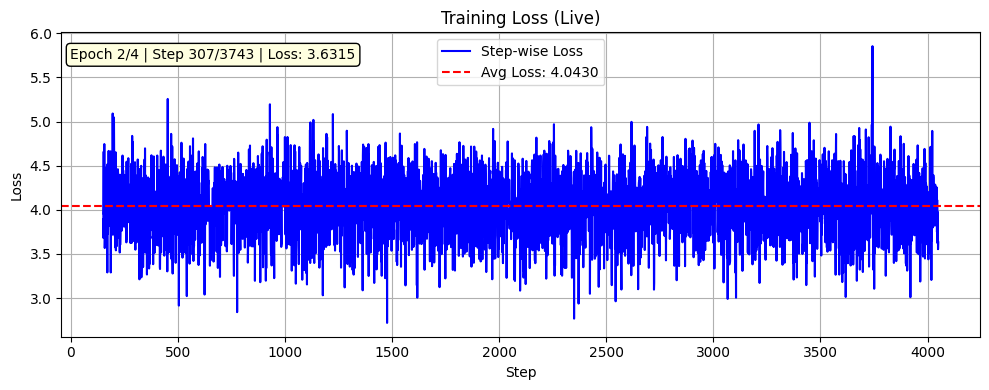
\includegraphics[width=0.8\linewidth]{Tuning.png}
\caption{Model training}
\end{figure}

\section{Evaluation and Results}
Performance is evaluated using four metrics across all languages. The table below summarizes multilingual evaluation.

\begin{table}[h]
\centering
\caption{Multilingual Model Performance}
\begin{tabular}{lcccc}
\toprule
Language & Accuracy & Precision & Recall & F1-score \\
\midrule
English  & 97.5\% & 96.8\% & 97.3\% & 97.0\% \\
Spanish  & 96.1\% & 95.6\% & 95.9\% & 95.7\% \\
French   & 95.8\% & 95.0\% & 95.4\% & 95.2\% \\
Hindi    & 94.5\% & 94.0\% & 93.8\% & 93.9\% \\
\bottomrule
\end{tabular}
\end{table}

\begin{figure}[h]
\centering
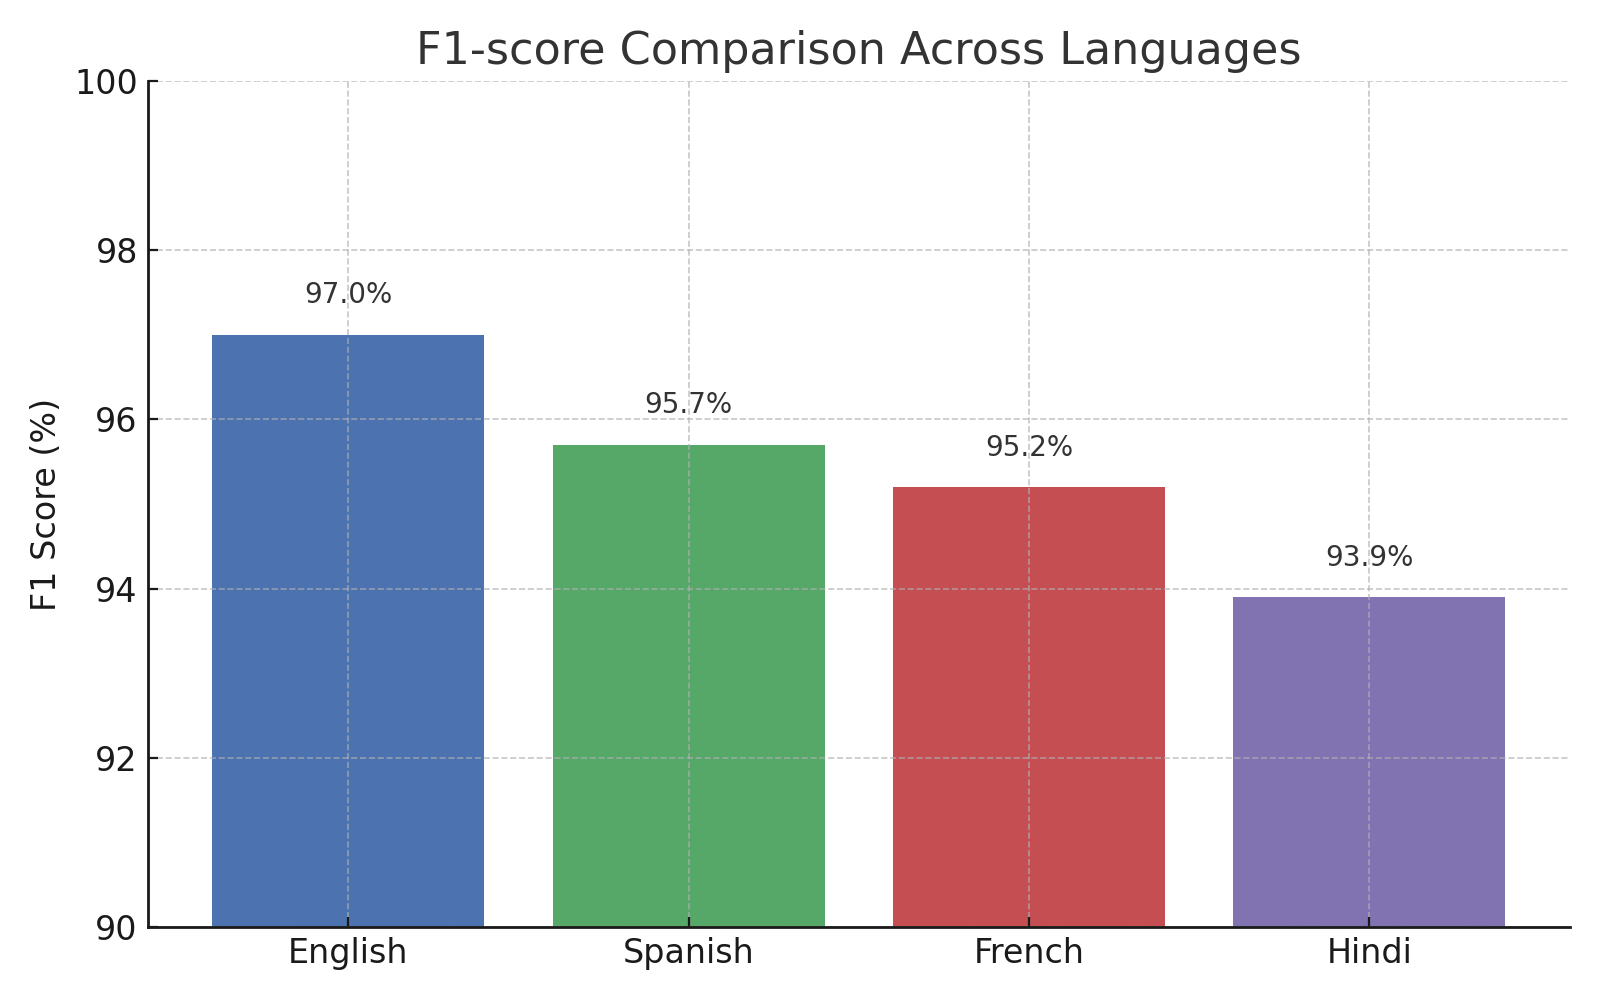
\includegraphics[width=0.8\linewidth]{f1_chart.png}
\caption{F1-score comparison across languages}
\end{figure}

\section{Conclusion}
The fine-tuned mBERT model achieves high accuracy and balanced performance across diverse languages. It demonstrates that transformer-based multilingual models are effective and scalable for cross-lingual intent classification in real-world NLP applications.

\ack This work was submitted as part of the DA 225o Deep Learning course project (Summer 2025), Indian Institute of Science, Bengaluru.

\bibliographystyle{ecai}
\begin{thebibliography}{}
\bibitem{} Devlin, J. et al. BERT: Pre-training of Deep Bidirectional Transformers for Language Understanding. NAACL, 2019.
\bibitem{} Conneau, A. et al. Unsupervised Cross-lingual Representation Learning. NeurIPS, 2019.
\bibitem{} Larson, S. et al. An Evaluation Dataset for Intent Classification and Out-of-Scope Prediction. EMNLP, 2019.
\end{thebibliography}

\newpage
\section*{Team Contributions}
\begin{itemize}
\item \textbf{Abhishek Gupta}: Training and model implementation
\item \textbf{Bharat Karthi R K}: Evaluation and result analysis
\item \textbf{Gayathri Ramasubramaniyam}: Dataset preprocessing
\item \textbf{Harikrishnan C}: Visualization and charts
\item \textbf{Indrerjit Singh Chahuan}: Literature review and writing
\item \textbf{Monika Tyagi}: Model optimization and documentation
\end{itemize}

\end{document}
